\begin{figure}
    \centering
    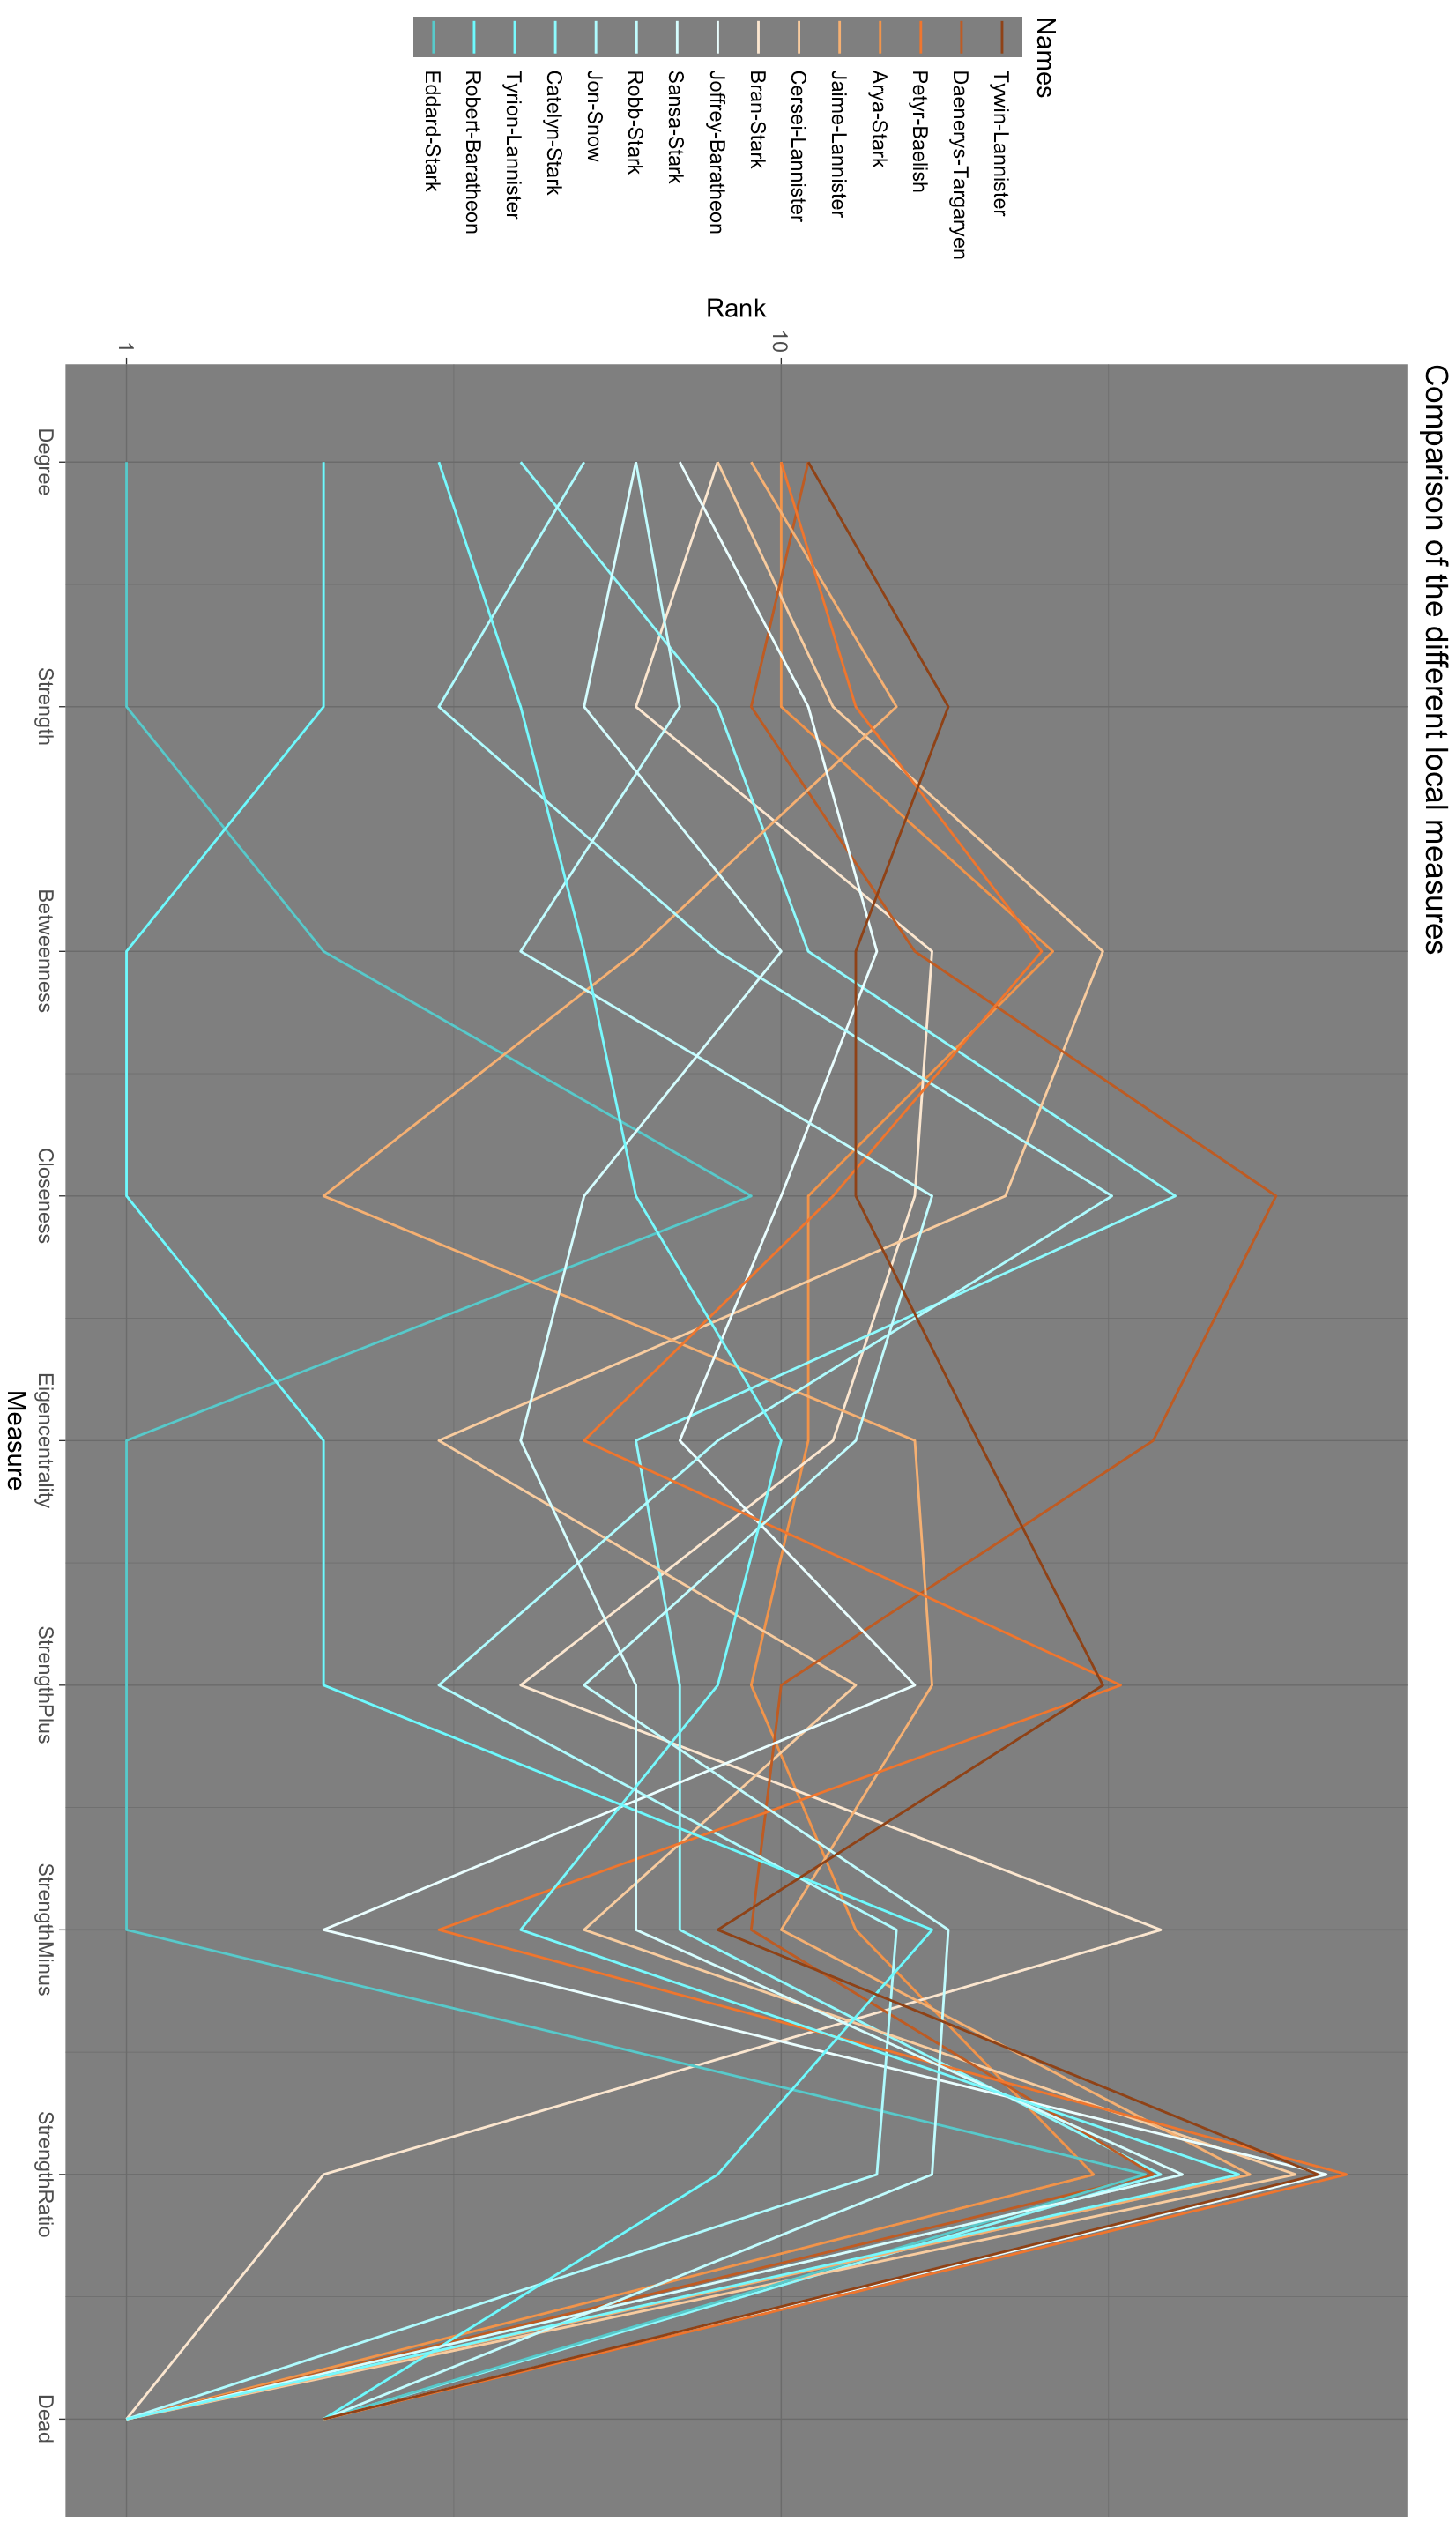
\includegraphics[scale=0.34]{plots/measurecomparison.png}
    \caption{The 15 characters with the highest degree are ranked across different local measures that somewhat represent influence and connectedness. For a better overview, a logarithmic scale was chosen. \textit{StrengthPlus} and \textit{StrengthMinus} only take the positive or negative relationships into account, hence \textit{StrengthRatio} is the ratio of the two. As the bottom of the graph usually represents a better ranking, alive characters correspond to 1, dead characters to 2 on the \textit{Dead} scale.}
    \label{fig:measurecomparison}
\end{figure}


\begin{table}
\caption{Centrality comparison of the 15 characters with the highest degree, corresponding to figure \ref{fig:measurecomparison}. The table gives away the ranks of the characters in a certain centrality measure.}
    \label{table:comparison}
    \begin{adjustbox}{angle=270}
    \begin{tabular}
    {p{2.5cm}p{0.9cm}p{1.2cm}p{1.2cm}p{0.9cm}p{1.2cm}p{1.2cm}p{1.2cm}p{1.2cm}p{0.9cm}}
    \toprule
    Names & Degree & Strength & Between-ness & Close-ness & Eigen-centrality & Strength Plus & Strength Minus & Strength Ratio & Dead\\
    \midrule
    Eddard-Stark & 1 & 1 & 2 & 9 & 1 & 1 & 1 & 36 & 0\\
    Robert-Baratheon & 2 & 2 & 1 & 1 & 2 & 2 & 17 & 8 & 0\\
    Tyrion-Lannister & 3 & 4 & 5 & 6 & 10 & 8 & 4 & 50 & 1\\
    Catelyn-Stark & 4 & 8 & 11 & 40 & 6 & 7 & 7 & 38 & 0\\
    Jon-Snow & 5 & 3 & 8 & 32 & 8 & 3 & 15 & 14 & 1\\
    \addlinespace
    Robb-Stark & 6 & 7 & 4 & 17 & 13 & 5 & 18 & 17 & 0\\
    Sansa-Stark & 6 & 5 & 10 & 5 & 4 & 6 & 6 & 41 & 1\\
    Joffrey-Baratheon & 7 & 11 & 14 & 10 & 7 & 16 & 2 & 68 & 0\\
    Bran-Stark & 8 & 6 & 17 & 16 & 12 & 4 & 38 & 2 & 1\\
    Cersei-Lannister & 8 & 12 & 31 & 22 & 3 & 13 & 5 & 61 & 1\\
    \addlinespace
    Jaime-Lannister & 9 & 15 & 6 & 2 & 16 & 17 & 10 & 52 & 1\\
    Arya-Stark & 10 & 10 & 26 & 11 & 11 & 9 & 13 & 30 & 1\\
    Petyr-Baelish & 10 & 13 & 25 & 12 & 5 & 33 & 3 & 73 & 0\\
    Daenerys-Targaryen & 11 & 9 & 16 & 57 & 37 & 10 & 9 & 37 & 1\\
    Tywin-Lannister & 11 & 18 & 13 & 13 & 20 & 31 & 8 & 66 & 0\\
    \bottomrule
    \end{tabular}
    \end{adjustbox}
\end{table}
